%%%%%%%%%%%%%%%%%%%%%%%%%%%%%%%%%%%%%%%%%%%%%%%%%%%%%%%%%%%%%%%%%%%%%%%%%%%%%%%%
%2345678901234567890123456789012345678901234567890123456789012345678901234567890
%        1         2         3         4         5         6         7         8


\documentclass[a4paper, 10pt, conference]{IEEEtran}
\usepackage{blindtext, graphicx}
\usepackage{listings}
\lstset { %
    language=C++,
    numbers=left,
    breaklines=true,
    xleftmargin=4em,
    resetmargins=true,
    basicstyle=\footnotesize,
    numberstyle=\footnotesize,
}
\usepackage{graphicx}
\usepackage[font=small]{caption}
\usepackage[utf8]{inputenc}

\graphicspath{ {./img1.png} }

\let\ACMmaketitle=\maketitle
\renewcommand{\maketitle}{\begingroup\let\footnote=\thanks \ACMmaketitle\endgroup}


%\overrideIEEEmargins
% See the \addtolength command later in the file to balance the column lengths
% on the last page of the document

% The following packages can be found on http:\\www.ctan.org
%\usepackage{graphics} % for pdf, bitmapped graphics files
%\usepackage{epsfig} % for postscript graphics files
%\usepackage{mathptmx} % assumes new font selection scheme installed
%\usepackage{times} % assumes new font selection scheme installed
%\usepackage{amsmath} % assumes amsmath package installed
%\usepackage{amssymb}  % assumes amsmath package installed

\title{Visual Line Following with Parrot MAMBO FLY Mini Drone}

% author names and affiliations
\author{
\IEEEauthorblockN{Emilija Kastratović}
\IEEEauthorblockA{Institute of Embedded Systems/Real-Time Systems\\Faculty of Engineering, Computer Science and Psychology\\Ulm University, Germany\\Email: emilija.kastratovic@uni-ulm.de\\Student ID number: 1052407}
}

\begin{document}

\maketitle

\pagestyle{plain}



%%%%%%%%%%%%%%%%%%%%%%%%%%%%%%%%%%%%%%%%%%%%%%%%%%%%%%%%%%%%%%%%%%%%%%%%%%%%%%%%
\begin{abstract}
The following paper proposes an implementation of a visual line following drone in MATLAB / SIMULINK. The task is to have the Parrot MAMBO FLY Mini Drone with its embedded camera at the bottom successfully follow a predefined red line on a flat green surface at a variable flying height. The camera’s viewfinder is split into three artificial sensors whose position is determined automatically in accordance to the height, and constant yaw adjustments depending on the sensors’ input turn the drone to the desired direction while flying at a constant speed. Simulation showed that the drone could successfully maneuver any path at a low height; however, higher heights propose a problem to the drone’s balance. This technique is easy to apply to other applications, such as transportation and infrastructure.\\\par
Keywords: line following, automatic sensor, vision-based\\

\end{abstract}
%%%%%%%%%%%%%%%%%%%%%%%%%%%%%%%%%%%%%%%%%%%%%%%%%%%%%%%%%%%%%%%%%%%%%%%%%%%%%%%%

\section{Introduction}
Line following robots and drones are one possibility to change mobility. Environmental and economic factors are the main reasons why such technology should be developed and used further. Today’s transportation means like highways, and train tracks are susceptible to environmental influences, resulting in high expenses and long works if damaged or renovated. A solution to this problem is automated line following drones and robots, which would cut infrastructural costs and reduce traffic risks for humans. Such an approach is already in use today, for example, in industrial manufacturing processes where line following robots are used in automated transportation of goods and materials. \cite{8679260} 
For this research, the Parrot MAMBO FLY Mini Drone will be used, which has a camera embedded on the drone’s bottom. Under reasonable lighting conditions, it will follow a flat, red line with a constant width on a green ground. The drone will be able to disregard the height it is flying on by automatically adjusting the sensor position. This project is done in MATLAB and Simulink using the Parrot Mini Drone Competition as a template for the drone’s model. The main implementation is done in the Flight Control System, namely the Image Processing System and the Path Planning system.\\\par
The main concepts this paper will focus on are how splitting the camera input into smaller squares is done, how the automatic selection of sensor squares according to the drone’s height works, and what is necessary to have the drone adjust its yaw in small, repeated nudges according to the sensor detection.\par

\section{Related Works}
A.H. Ismail et al. \cite{5356366} have implemented a vision-based system for a line following mobile robot. They used a low-cost webcam as the sensor and processed the resulting output by segregating the necessary information and supplying it to the robot’s controller. Technical limitations also included the resolution and image quality and restricting themselves to a white line on a dark green floor. The resulting processed image is also set in grayscale and could be represented as a matrix consisting of ones and zeroes, with one indicating the white line. Similarly to this research, the image and thus the matrix was obtained by using thresholds to determine whether any block of the matrix is considered to have a significant amount of white pixels, resulting in a one in the matrix block.
M.S.B. Mostafa et al. \cite{8679260} proposed an amphibious line following robot that works on both land and in water. It should help solve the problem of delivery and transportation in the context of Bangladesh, which is an area prone to flooding. It follows a predetermined white line on a dark surface. Their sensor, however, is an IR sensor whose LED emits an infrared ray. Again, using a threshold, the robot can sense the line. An approach using an infrared ray is superior to using a camera, as lighting conditions can be disregarded.\\\par
Both pieces of research, too, approach the problem using low cost and easy to install components. This furthermore supports the aforementioned proposal of low costs and easier transportation, thus making infrastructure easier to maintain.\\
This research differs in the type of hardware that is used and should show that implementing such an application can be done for any kind of robot. In addition, it emphasized that different types of transportation are viable and can and should be implemented more.


\section{Concept}
The Parrot MAMBO FLY Mini Drone will be used to follow a line. It will do so by flying forward continuously while using the camera on the bottom to detect the line’s direction and adjust its yaw accordingly to stay on the line. The drone will also be able to follow the line independently from its flying height. Because this line following algorithm must work with a variable flying height of the drone, the line which the drone follows needs to lie flat on the ground, have a fixed and continuous width and have a different color from the ground. In this research, a 10cm wide, red line on a green ground is used. Red and green are the colors used because they are complementary colors with the starkest contrast, which helps in the threshold determination, thus making them the easiest to work with.
In the beginning, the drone is being positioned on the line it is supposed to follow and the target height is given to the drone. Even though the flying height can vary during its course, for simulation purposes, the drone will fly at a predetermined, constant height. The drone is flying at a constant speed at all heights. The only factor determining the speed is whether the drone can make yaw adjustments in time and not fly over the line.\\

\subsection{Sensor}
The camera is the critical component for the line following algorithm. It can distinguish RGB colors. It will be used to emulate artificial dynamic sensors using a single camera sensor. This is done by selecting specific squares of that viewfinder. For this, the entirety of the 120px by 160px viewfinder of the camera input is used. From this input, two 10px by 10px squares in the middle of the upper third of the image are selected. Those automatically determined squares left, and right to the red line will create the sensor made up of said smaller sensor subunits. It is crucial the sensors have some space next to the line, as having them be right next to the line will lead to unwanted behavior of the drone. For example, environmental factors like wind or initial balancing problems of the drone would have the sensor unwantedly detect the red line. An additional sensor subunit is selected right underneath the red line, ensuring that the drone is on the path. If that sensor does not detect red, the drone will stop flying. It is beneficial to have those squares in the upper third of the input as the drone can make its yaw adjustments in time before the curve. This time buffer that is then created allows a smoother flight and turn. The drone can already adjust while already flying forward, resulting in a smoother transition and adjustment into the curve.\\\par
The sensor can enter two states to which the drone will respond accordingly.
The first one is the base case; both the left and right sensor squares are detecting green (i.e., not the red line), and the sensor in the middle is detecting red. This is the state the drone will try to always achieve and return to.
The second case occurs when a curve is coming up. Either square on the side is now detecting red. Depending on whether it is the left or right square that detects red color, the drone will adjust its yaw to the left or right, respectively, in small, repeated nudges to return to the base case. While this is happening, the drone will continuously be flying forward. This is the mechanism that allows the drone to follow the line.
It should be mentioned that the accuracy of this mechanism increases with a higher number of smaller subunits. Note that the single input of this given small RGB camera only allows a modification of the 120px x 160px input. Additionally, the need for splitting proposed another challenge for this concept.
Implementation in Simulink is done by using three Selection blocks with which it is possible to select a specific area of that viewfinder. Those three selection blocks make up the square sensor subunits.\\
\begin{figure}
    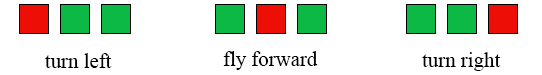
\includegraphics[width=\linewidth]{fig1.jpg}
    \caption{Visualization of the sensor subunits}
    \label{fig:my_label}
\end{figure}


\subsection{Automatic Sensor Position Determination Depending on Flying Height}
The drone’s flying height automatically determines the two 10px x 10px sensors’ vertical position. The horizontal position is set in the upper third of the viewfinder for easier curve maneuvering, as explained before. The additional sensor in the middle of its position will not be changed, as its only purpose is ensuring the drone is on the path. For the sensors to work and conduct a correct signal, the color threshold must be adjusted. 
At first, the RGB image from the camera is obtained to use the respective red, green, and blue channels of the image. The red is filtered with this operation \cite{3}:\\
\begin{equation}
     R - (B/2) - (G/2)
\end{equation}\par

With the z value defining the drone’s flying height, it is possible to determine the distance the sensors must have from the middle. This approach uses a variable height as the sensor determination factor is more comfortable to implement than a variable width. Having explained that the sensors need to have a certain amount of space next to the line, detecting that needed space is much more complicated as space would increase with increased width. Thus, with this method, knowing that the line has a fixed width, space can also stay constant, so the only thing that needs to be adjusted is the position of the two horizontal sensors. \\\par
They need to be adjusted because with increased height, the line width decreases for the viewfinder. If the sensors then detect the red signal too late, the drone would not adjust in time. To counter this, the sensors move closer together with increased height. Threshold can be at a constant value.
Technical limitations of this drone model allow for the lowest height to be 1 meter above the ground and the highest height 1.5 meters. In general, if the drone can adjust fast enough and the image detection threshold for the red color is sensitive enough, the drone can fly at any height above 1 meter.\\

\subsection{Yaw Adjustment}
A drone following a line is, at its basis, just changing its x and y coordinates. Modifying the drone’s roll and pitch is thus not required; however, there are advantages to adjusting its yaw.
First is an easier change of direction, for example, when maneuvering curves. The second is always having the drone face forward, allowing the sensor to always be at the drone’s front. This makes implementing the sensor much more comfortable, as its horizontal position can always stay the same (vertical position is changed by height adjustment).
Two things need to be done. First, the drone will have to know what position to fly to while always facing forward. Using simple trigonometry, this can be expressed as following in pseudocode:
\begin{equation}
    x_{pos} = x_{pos} + cos(yaw) \cdot gain
\end{equation}
\begin{equation}
     y_{pos} = y_{pos} + sin(yaw) \cdot gain
\end{equation}\par
The drone now flies to the given position, but the yaw still needs to be adjusted.
Depending on whether the left or right sensor subunit detects an input, a constant signal is conducted until the sensors reach the base case again. During this signal, the drone’s yaw changes in small, repeated nudges.\\


\section{Implementation}
Implementation is done in MATLAB / Simulink using the parrotMinidroneCompetition project as a template. For the line following algorithm, only the Image Processing System and the Path Planning subsystem in the Control System are modified. Image Processing System is used for the sensor, and the Path Planning system handles speed, drone movement, direction, and yaw control.\\

\subsection{Image Processing System}

\begin{figure}[t]
    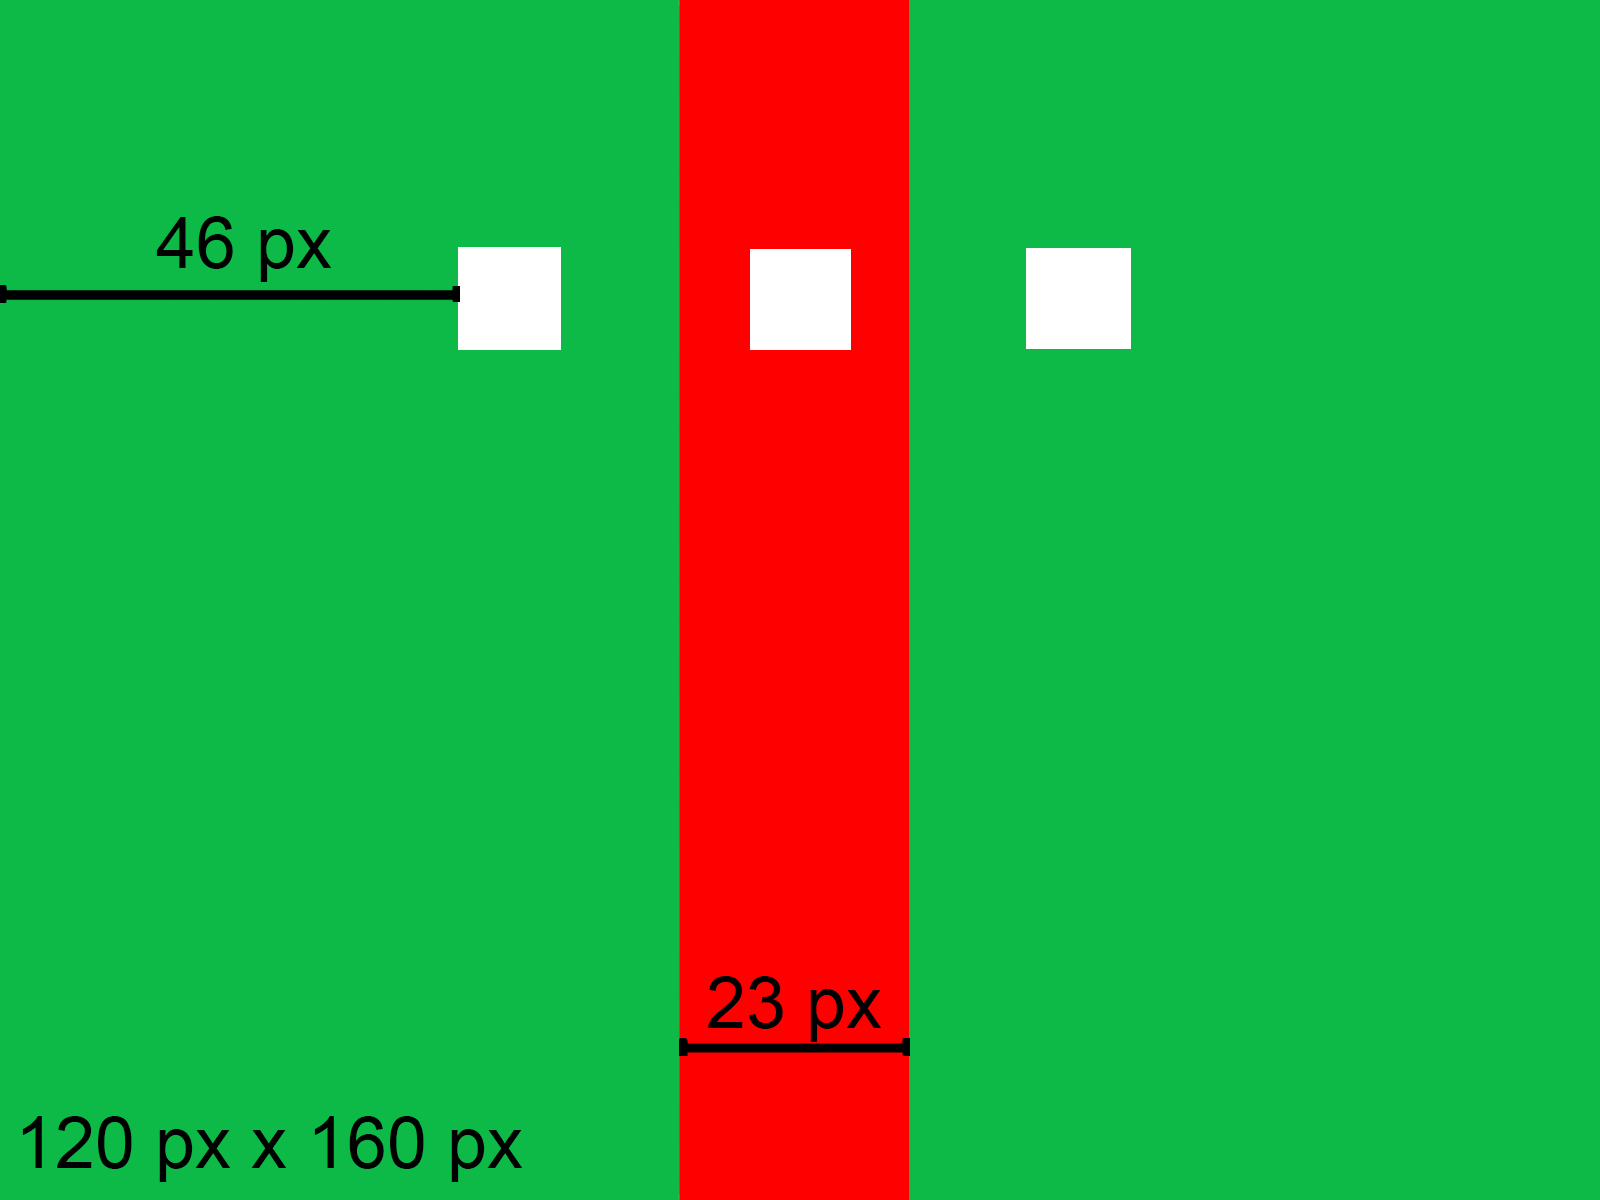
\includegraphics[width=121px, left]{sensor.jpg}
     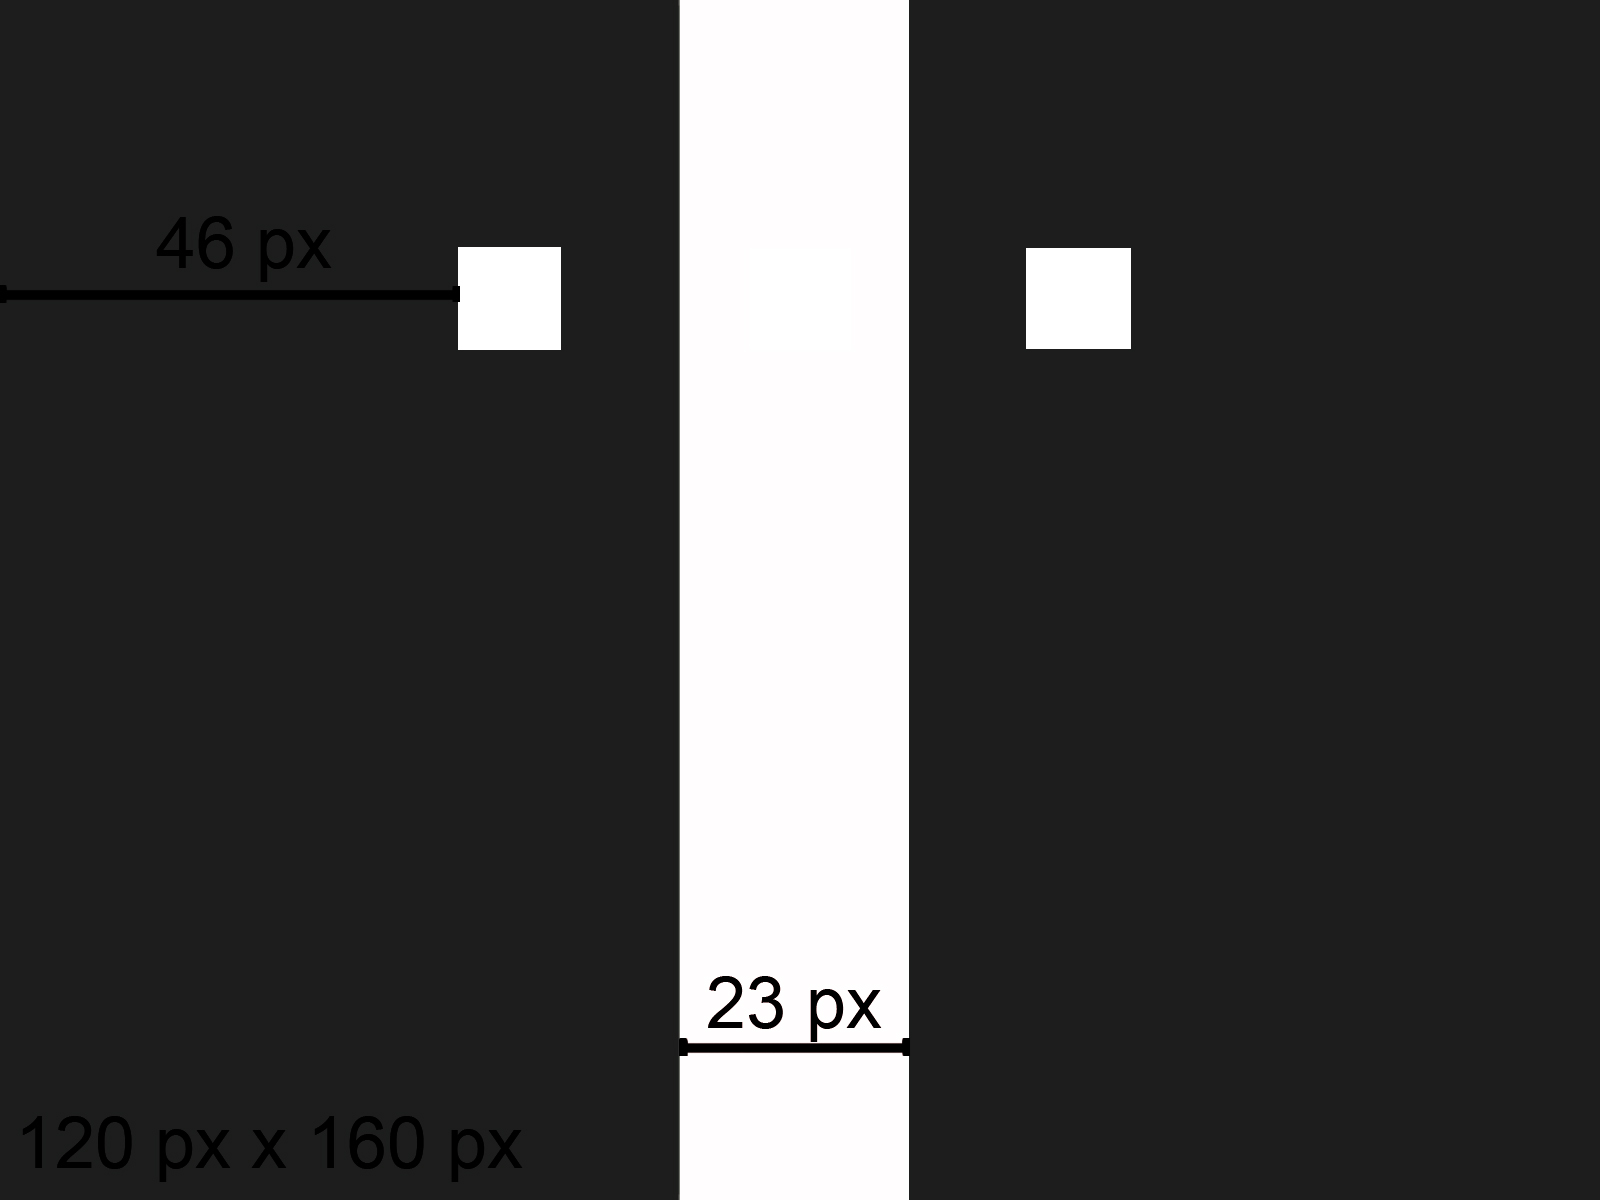
\includegraphics[width=121px, right]{sensor-red.jpg}
    \caption{Image Viewfinder before and after filtering the red channel. }
    \label{fig:my_label} 
\end{figure}

The IPS receives a picture input from the drone’s camera. A Parrot Image Conversion block then converts the Y1UY2V color space of the input image to RGB color space and outputs a 120px by 160px array of type uint8 for each of the selected RGB color components \cite{1}. Additionally, the RGB channels are input to a video viewer (viewfinder).
Equation (1) is used to filter the red channel. The color channel of an image is a grayscale image with lighter areas corresponding to a higher amount of that color and, in return, darker areas implying a smaller amount of the chosen color, i.e., the luminance value of the chosen color are shown (Fig. 2). Since the luminance value for red is 54, an initial threshold of greater than 50 (already given) is chosen to eliminate all darker pixels of the color channel image, i.e., all colors except pure red are filtered out. If pixels pass this threshold, the sum of their luminance value is used further to determine whether the area contains enough red color, accomplished by a threshold of greater than ten that was chosen through simulation and testing. In conclusion, if the image is considered to contain enough red color, the signal will be conducted.
Using Selector blocks in Simulink, it is possible to restrict this process to any area. Selecting areas of 10px by 10px in the upper third of the image creates the artificial sensor. The sensors’ optimal positions can be represented with two linear functions (Fig. 3). The functions were determined measuring the optimal distance between the sensor and using the picture from the camera’s viewfinder.
\begin{figure}
    \centering
    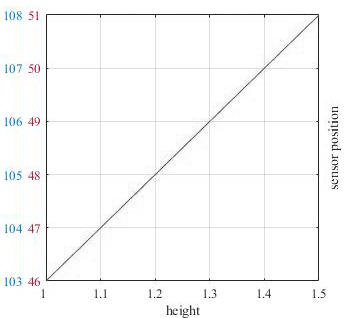
\includegraphics[width=160px]{graph.jpg}
    \caption{Sensor Position Depending on the Drone Height. Red and blue numbers represent the left and right sensor respectively}
    \label{fig:my_label} 
\end{figure}
The middle 10px by 10px sensor is set in the middle of the two outer sensors.
In the end, three signals are used for the sensor. Each of those signals is then “muxed”, i.e., put into a Mux block – Multiplex scalar or vector signals – to output the signal to the Path Planning system.\\

\subsection{Path Planning}
Signals sent by the IPS are “demuxed”, i.e., vector signals are split into scalars \cite{2} in the Path Planning system. Three signals are necessary; left (by the left sensor subunit), middle (by middle sensor subunit), and right (by the right sensor subunit).
First the drone's ascends to the target height, that is given to the drone before the simulation starts. The sensor then will only transmit the signal after two seconds, because otherwise the yaw subsystem would already be triggered when it should stay idle.
The drone will be flying forward if it detects a signal from the middle subunit. This prevents the drone from keep flying if it reaches the end of a path. A constant gain of 0.0003 was chosen through simulation and testing. This value is constantly added to the drone's position, making it the drone's speed. Any greater value would result in too little time for the drone to adjust its orientation, making it fly over the line. This gain value is used in equations (2) and (3) to determine the drone's x and y position (without the yaw adjustment).\\\par
Two subsystems, ‘direction’ and ‘yaw’ handle which direction (left or right) and how much the drone must adjust its yaw.
In the ‘direction’ subsystem, three constants (-1, 0, 1) in addition to two switches are used to determine the direction. ‘Direction’ outputs a value to ‘yaw’. If that value is either -1 or 1, the drone will change its yaw to the left or right, respectively, else, 0 is output, and the drone’s yaw will not change. In the base case, 0 is being output; however, if either square receives an input, the switch will send the respective constants. Their sum defines what constant is being sent through. In an impossible case where both left and right signals are detected, the drone would fly forward since their sum equals 0.
The ‘yaw’ subsystem is activated using a trigger event. This trigger event is a sine wave signal sent when either the left or right subunit discerns a signal. It is crucial the signal be repeated continuously because otherwise, the trigger even would only happen once. At every sine wave peak (so when the sine of the signal is equal to 1, a signal is being sent, continually triggering the ‘yaw’ subsystem.
When triggered, the ‘direction’ value is put in a switch with two constants of -0.31 and 0.31. Those values were determined using simulation and testing. This constant is then added to the previously mentioned yaw. This sum value is then used in equation (2) and (3) and set as the new yaw value.Any value greater than 0.31 would result in too big of a yaw adjustment, meaning the drone would be adjusting in a zigzag pattern when encountering a curve, leading to instability and rough curve maneuvering. Any value less than 0.31 would be too small of a yaw adjustment, making the drone fly over the line while adjusting.
Finally, the x, y, and height values are put into a Mux, converted to a single data type, and set as the position reference value, and the yaw value is set as the orient reference value in the Bus Assignment Block.\\ 


\section{Evaluation}
Extensive testing through simulation was done to determine the optimal values for each height. However, the technical limitations of the Parrot MAMBO FLY Mini Drone proposed many difficulties.
This concept with this drone works best at the height of 1.1 meters above the ground. That is also when the sensor at the bottom of the drone is at an optimal height and performs best. For that, a predetermined course that features different types of curves was chosen to test this implementation. Turns such as elongated curves, rounded 90°, and U-turns were chosen to simulate common infrastructure, whereas 90° corners and a curved zig-zag pattern was added to test more difficult paths.\\\par
The simulation showed that the drone managed to follow the line almost perfectly at that height with the variables mentioned earlier. 
Problems arose when the drone came off a curve onto a straight path; the drone will not always adjust exactly straight onto the line but sometimes fly in a very light zig-zag like pattern while continually adjusting. A solution to this is more sensors at the drone’s front that would adjust the drone’s yaw ever so slightly to correctly follow the path.
Another problem was the drone’s balance while turning. The yaw adjustment is punctual, not continuous, and very quick. This will always result in an unstable and swinging drone if repeated often and at an increased height, the drone will become more unstable the more it makes subsequent turns. The turns as mentioned above chosen in the course are not optimal for the maximum height of 1.5 meters and will result in the drone swinging excessively.
A solution to this is a course featuring less tight turns, or a slower speed or smaller, but more rapid yaw adjustments. However, the latter option was impossible to implement because SIMULINK does not have an option for a variable gain based on input. An attempt was made to set the yaw constant with a function, similarly to how the sensors are adjusted. However, no optimal function was found that works for all heights because a smaller yaw adjustment implies a slower speed.
The biggest problem continues to be the decrease in balance with each turn which cannot be solved even with minimal yaw adjustments.\\



\section{Conclusion}
With this project, the goal was to implement a line following drone flying at a variable height. This was done using the drone’s camera, splitting the viewfinder to create subunits that make up a sensor and can adjust their vertical position in relation to the drone’s height. The drone would then be flying forward and continuously adjusting its orientation in small, repeated nudges. Implying the drone would always have a front side, this improves ease of curve maneuvering.
More automatic adjustments would make the drone even more useful, such as adjusting to the line’s width, color, and flexible heights and more fine-tuning is needed to have the drone fly more securely at higher heights.\\\par
Use cases for this are mainly improved and easier transportation. Areas around the world that require a fast, easy and cheap means of transportation could benefit from such a technology. Infrastructure could be supplemented with simple lines painted on the floor, abolishing the need for costly roads and train tracks requiring tedious maintenance.\\


\addtolength{\textheight}{-12cm}

\bibliography{ref}
\bibliographystyle{IEEEtran}  

\end{document}
